\documentclass{anstrans} \usepackage{amsmath} \usepackage{amssymb}
%\usepackage{amsthm}
\usepackage{amscd}
%\usepackage{amsfonts}
\usepackage{graphicx}% \usepackage{fancyhdr} \usepackage{color} \usepackage{cite}

%\usepackage[T1]{fontenc} \usepackage[utf8]{inputenc} \usepackage{authblk}
\usepackage{physics} \usepackage{float} \usepackage{caption} \usepackage{subcaption}

\setlength{\columnsep}{0.5 in}

\newcommand{\expv}[1]{\ensuremath{\mathbb{E}[ #1]}} \newcommand{\xs}[2]{\ensuremath{\Sigma_{#1}^{(#2)}}}
\newcommand{\intO}{\ensuremath{\int\limits_{4\pi}}} \newcommand{\intz}{\ensuremath{\int\limits_0^1}}
\newcommand{\intf}{\ensuremath{\int\limits_{-\infty}^\infty}}
\newcommand{\intzf}{\ensuremath{\int\limits_{0}^\infty}}
\newcommand{\LargerCdot}{\raisebox{-0.25ex}{\scalebox{1.2}{$\cdot$}}}

%\textwidth6.6in \textheight9in


%\setlength{\topmargin}{0.3in} \addtolength{\topmargin}{-\headheight} \addtolength{\topmargin}{-\headsep}

%\setlength{\oddsidemargin}{0in}

%\oddsidemargin  0.0in \evensidemargin 0.0in \parindent0em

%\pagestyle{fancy}\lhead{MATH 579 (UQ for PDEs)} \rhead{02/24/2014} \chead{Project Proposal} \lfoot{}
%\rfoot{\bf \thepage} \cfoot{}
\title{Time-Dependent Sensitivity Analysis of OECD Benchmark using BISON and RAVEN}

\author{Paul W. Talbot$^{*}$, 
        CongJian Wang$^{\dagger}$, 
        Cristian Rabiti$^{\dagger}$,
        Kyle Gamble$^{\dagger}$,
        Anil K. Prinja$^{*}$}
        %TODO rest of raven team, bison team?
\institute{
  $^*$Department of Nuclear Engineering,
  University of New Mexico,
  Albuquerque, NM, 87131 
  \and 
  $^\dagger$Nuclear Engineering Methods Development,
  Idaho National Laboratory,
  Idaho Falls, ID, 83415}
  \email{talbotp@unm.edu }%\and prinja@unm.edu \and cristian.rabiti@inl.gov}
%\date{}


\begin{document}
\section{Introduction}
Developments in uncertainty quantification in nuclear simulations have decreased the computational cost
required to perform accurate sensitivity analysis \cite{cristiansmeared,ans2014,ans2016sum,physor2016}.
Implementation of these methods in the RAVEN \cite{raven} framework allows additionally for time-dependent
sensitivity analysis of uncertain input variables.  By demonstration we consider an OECD benchmark case (TODO
cite benchmark).  We propagate uncertainties in the input parameters using RAVEN operating on the BISON
\cite{bison} fuels performance code.  We then consider the time-evolution of the sensitivity of several output
responses to the uncertain input parameters.  We perform sensitivity analysis  using time-based stochastic 
collocation for generalized polynomial chaos (SCgPC) and high-dimension model reduction (HDMR) \cite{Ayres}.

\section{Methods}
TODO Describe OECD benchmark.

For propagation of uncertainty we make use of the high-dimension model reduction (HDMR) expansion,
\begin{equation}\label{eq:hdmr}
  u(Y) = u_0 + \sum_{n=1}^N u_1 + \sum_{n_1=1}^N\sum_{n_2=1}^{n_1-1} u_{n_1,n_2} + \cdots,
\end{equation}
where $u(Y)$ is the response as a function of inputs $Y=(y_1,\ldots,y_N)$, $N$ is the dimensionality of the
input space, and the components $u_i$ are defined as
\begin{equation}
  u_0 \equiv \int\cdots\int u(Y) dY,
\end{equation}
\begin{equation}
  u_1 \equiv \int\cdots\int u(Y) dy_2\cdots dy_N,
\end{equation}
\begin{equation}
  u_{1,2} \equiv \int\cdots\int u(Y) dy_3\cdots dy_N,
\end{equation}
and so forth.  Each of the terms in Eq. \ref{eq:hdmr} can be represented using a generalized polynomial chaos
expansion,
\begin{equation}
  u(Y) \approx \sum_{k\in\Lambda}c_k\Phi_k(Y),
\end{equation}
where $\Phi_k$ are multidimensional polynomials of order $k=(k_1,\ldots,k_N)$ and $\Lambda$ is a combination
of multi-indices corresponding to polynomial orders.  Scalar coefficients $c_k$ are approximated using
sparse-grid collation numerical integration cite{smolyak}.

\section{Results}\label{results}
In Figures \ref{fig:pct}-\ref{fig:elong}, the evolution of sensitivities of the various responses are shown
with respect to increasing burnup.  In addition, the power history used in the simulation is overlayed to
provide insight in time-based changes.  In each case, only the most significant uncertain inputs are shown
for clarity.

For both the max clad surface temperature and max fuel centerline temperature, one parameter (inlet
temperature and fuel conductivity respectively) dominates variance over most of the history; however, system
power is more impactful near gradients in the power profile.
\begin{figure}[H]
  \centering
  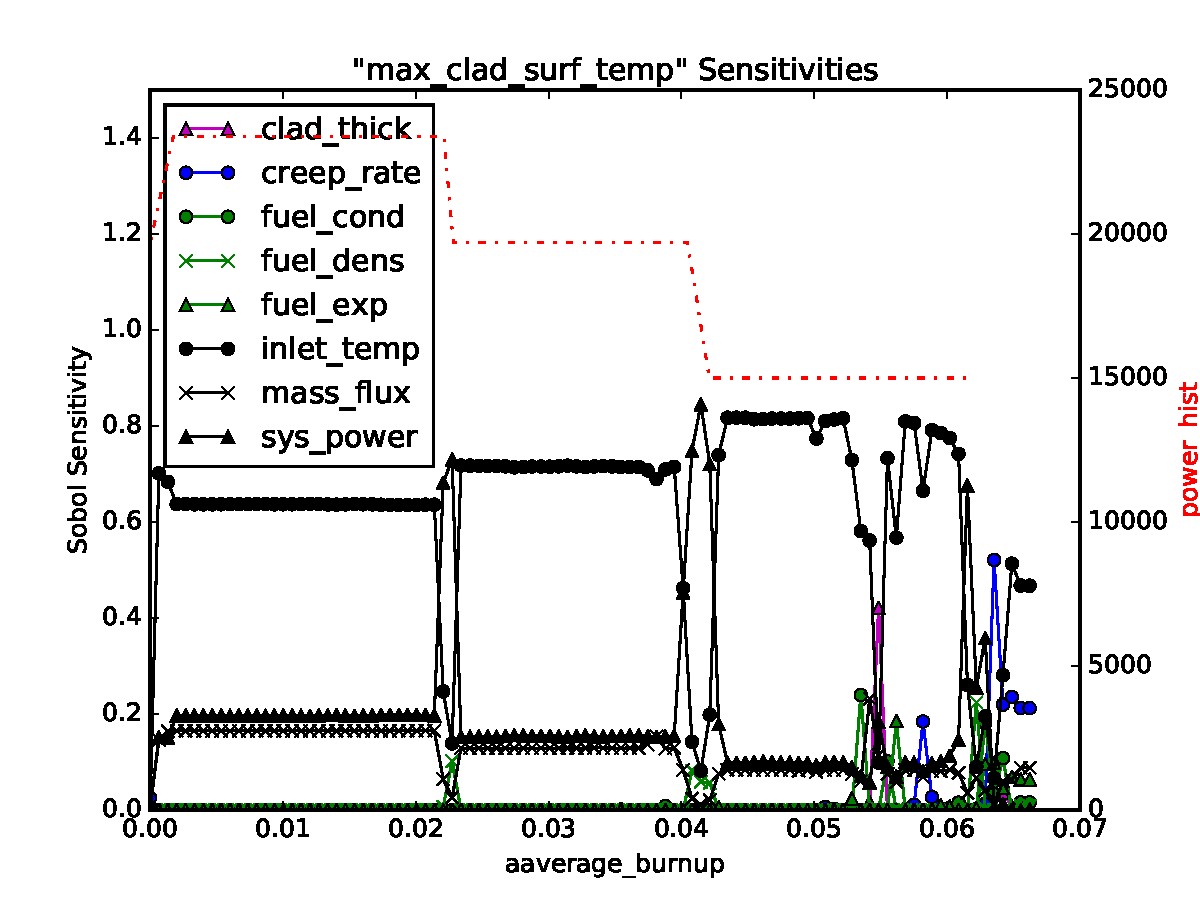
\includegraphics[width=\linewidth]{./sens_max_clad_surf_temp}
  \caption{Max Clad Surface Temperature}
  \label{fig:pct}
\end{figure}
\begin{figure}[H]
  \centering
  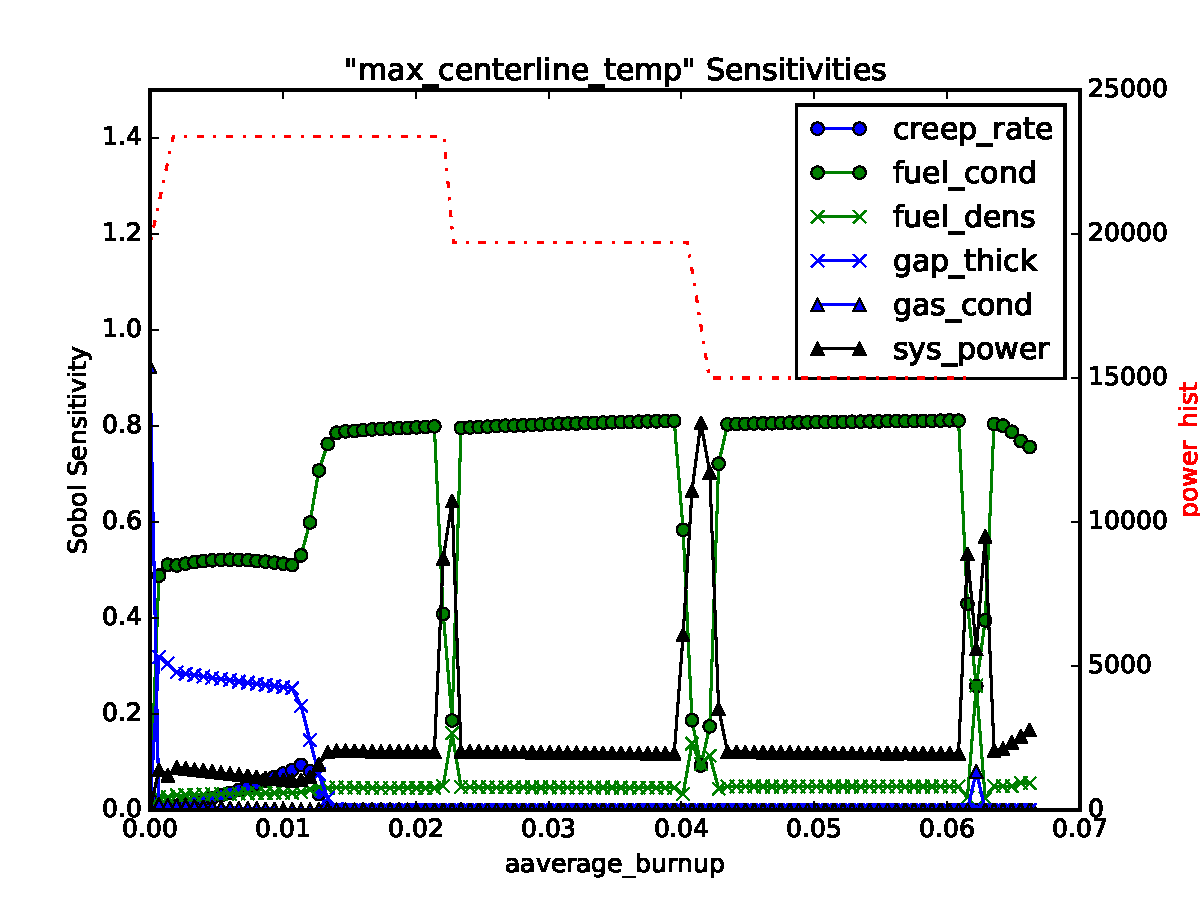
\includegraphics[width=\linewidth]{./sens_max_centerline_temp}
  \caption{Max Fuel Centerline Temperature}
  \label{fig:centerline}
\end{figure}
As expected, the clad creep rate is the most sensitive parameter for clad creep strain; however, it is
interesting to note the rise and fall of the gap thickness as an important parameter in the middle of the
burnup range.
\begin{figure}[H]
  \centering
  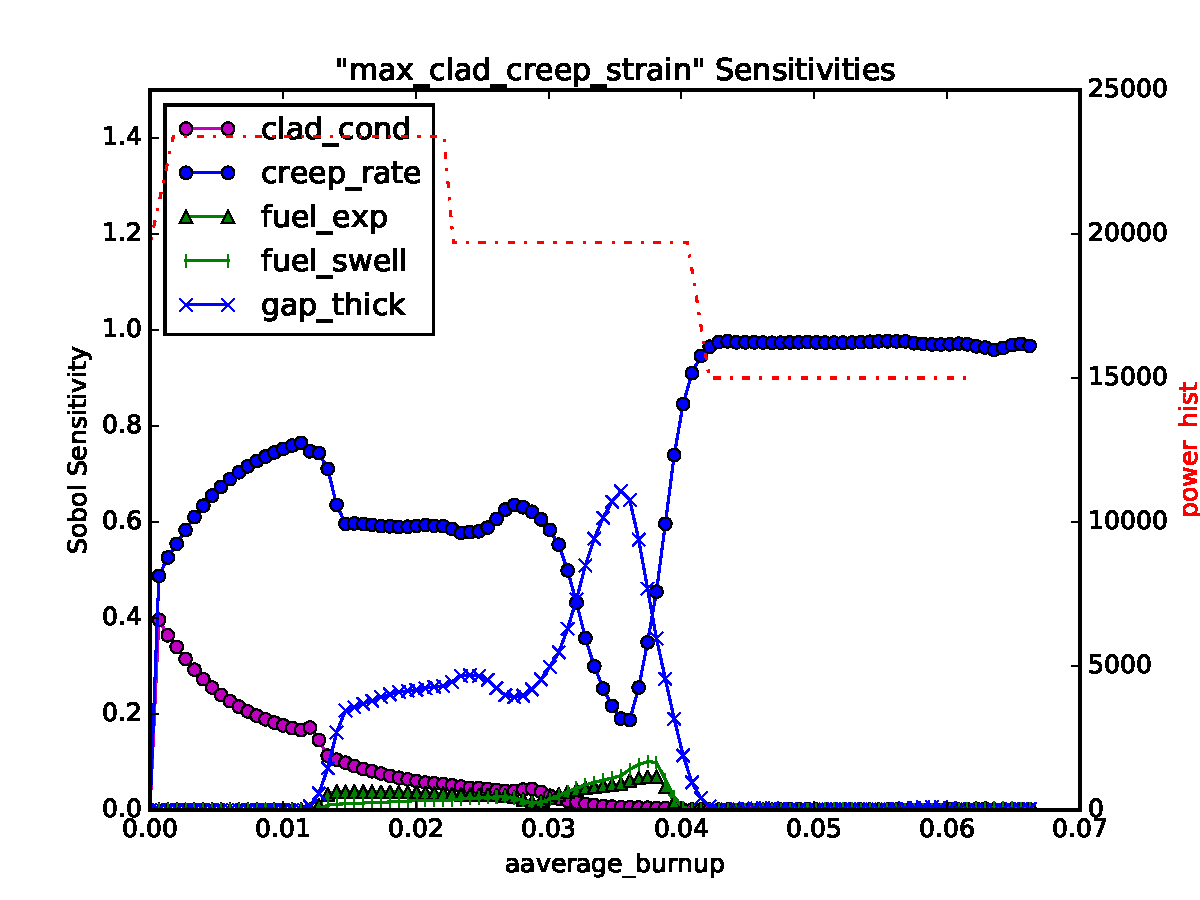
\includegraphics[width=\linewidth]{./sens_max_clad_creep_strain}
  \caption{Max Clad Creep Strain}
  \label{fig:strain}
\end{figure}
Early in life the fission gas release is dependent on several parameters, which gives way to only the fuel
conductivity and system power later.
\begin{figure}[H]
  \centering
  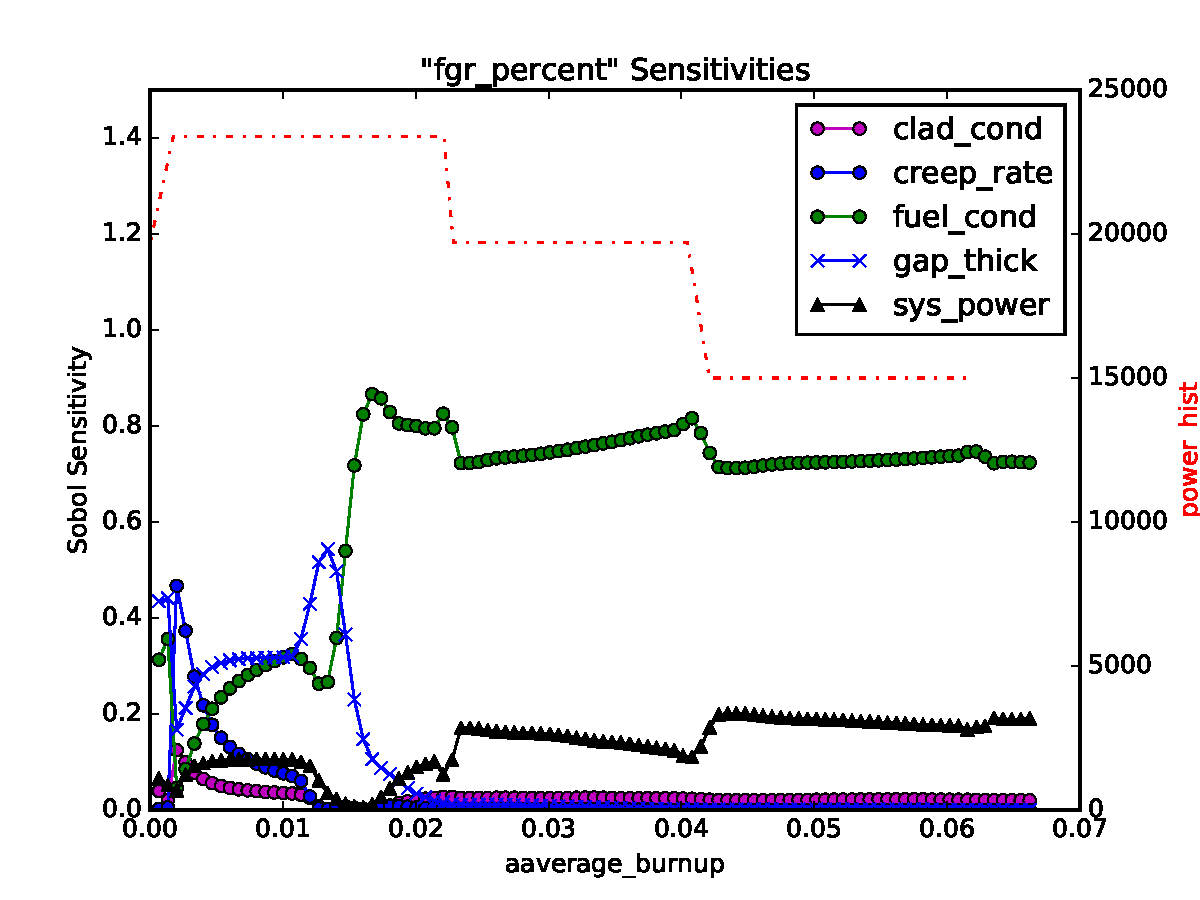
\includegraphics[width=\linewidth]{./sens_fgr_percent}
  \caption{Fission Gas Release (Percent)}
  \label{fig:fgr}
\end{figure}
The sensitivities in the variance of clad elongation have three distinct sections.  At the beginning, clad
elongation is perturbed most by clad conductivity, inlet temperature, and system power, with growing influence
from fuel density.  These are somewhat suddenly replaced by gap thickness, which then slowly trades places
with clad creep rate over the remainder of the life cycle.
\begin{figure}[H]
  \centering
  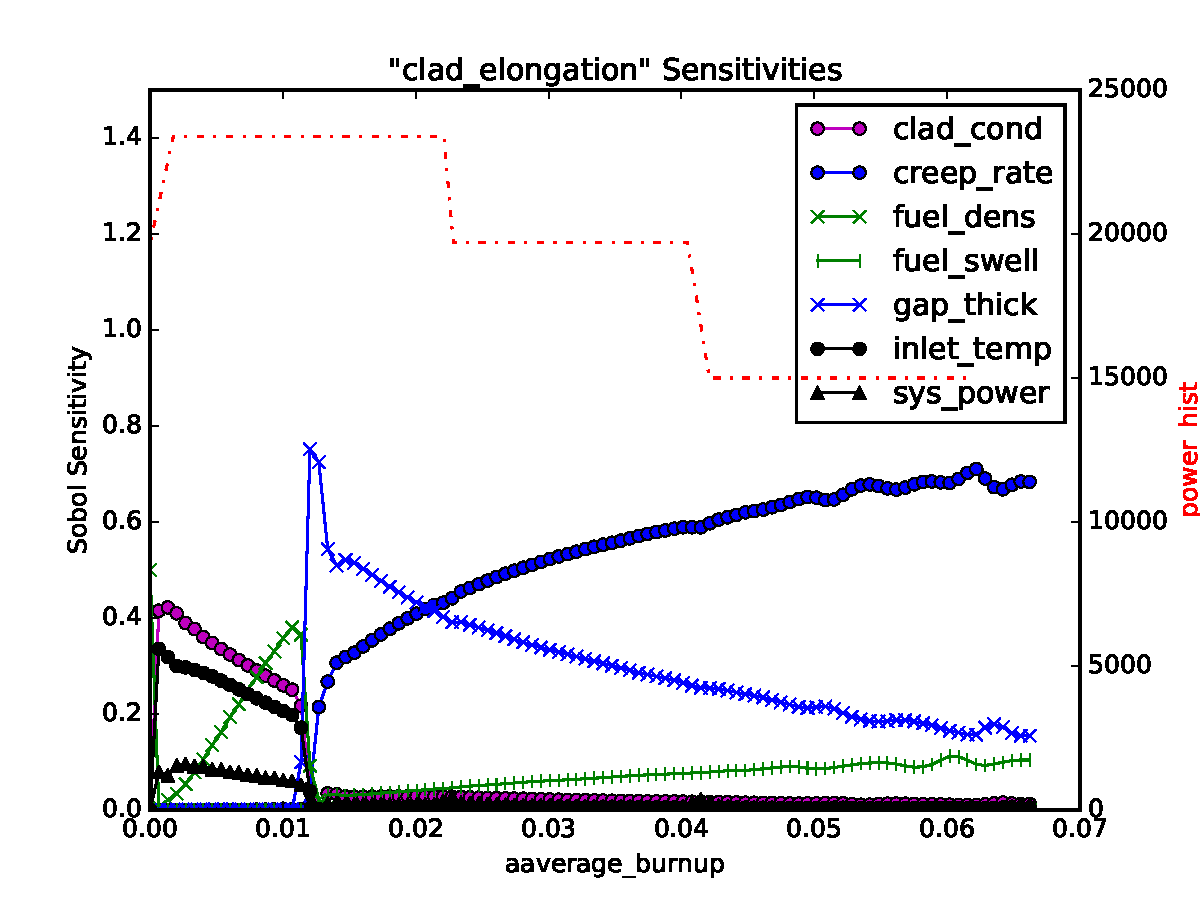
\includegraphics[width=\linewidth]{./sens_clad_elongation}
  \caption{Clad Elongation}
  \label{fig:elong}
\end{figure}


\section{Discussion}
We have demonstrated how HDMR and SCgPC can be used in RAVEN to perform time-dependent uncertainty propagation
analysis in codes modeling transient behavior.  Reviewing the time-evolution of Sobol sensitivities provides
new methods in understanding the impact of uncertain input parameters as changes occur during the transient
simulation.  At small additional cost to static uncertainty propagation, transient analysis has valuable
insights to offer.

\bibliography{../bibliography/uq}{}
\bibliographystyle{ans}
\end{document}
